\documentclass{article}

\usepackage[margin=.75in]{geometry}
\usepackage{amsmath}
\usepackage{amssymb}
\usepackage[shortlabels]{enumitem}
\usepackage{pgfplots}
\usepackage{float}
\usepackage{verbatim}
\usepackage{caption}
\usepackage{subcaption}

\usepackage{mathtools}
\DeclarePairedDelimiter\norm{\lVert}{\rVert}%

\author{Anthony Siddique, Damien Prieur, Jachin Philip, Obinna Ekeh}
\title{Homework 2\\ MEM 633 \\ Group 1}
\date{}

\begin{document}

\maketitle

\section*{Problem 1}
Given the following set of vectors
$$
\begin{bmatrix}
2-3j \\
1+4j \\
\end{bmatrix}
,
\begin{bmatrix}
8+2j \\
1+j \\
\end{bmatrix}
,
\begin{bmatrix}
j \\
5 \\
\end{bmatrix}
$$
\begin{enumerate}[a)]
\item Is the set independent over the field of the real numbers ($\mathbb{R}$)? Explain.
\newline
\newline
If the set is linearly dependent that means $\exists a,b \in \mathbb{R}$ such that
$$
a
\begin{bmatrix}
2-3j \\
1+4j \\
\end{bmatrix}
+b
\begin{bmatrix}
8+2j \\
1+j \\
\end{bmatrix}
=
\begin{bmatrix}
j \\
5 \\
\end{bmatrix}
$$
We can show there is no solution just by finding a solution for the first row and showing it doesn't work for the second
$$ a(2-3j) + b(8+2j) = j$$
Expanding and grouping the real and imaginary parts we get a system of equations
\begin{align*}
2a + 8b &= 0 \\
-3a + 2b &= 1 \\
\end{align*}
The first equation implies $a = -4b$ and substituting that into the second equation we get
$$ -3(-4b) +2b = 1 \implies 14b = 1 $$
So we have $ a = \frac{-2}{7}, \quad b = \frac{1}{14} $
Checking if the solution also works for the second row we get
$$ \frac{-2}{7}(1+4j) + \frac{1}{14}(1+j) = 5 $$
Just looking at the real parts we see the solution is not valid.
$$ \frac{-2}{7} + \frac{1}{14} \neq 5 $$
Therefore $\nexists a,b \in \mathbb{R}$ so the set is linearly independent over the field of real numbers ($\mathbb{R}$).

\item Is the set independent over the field of complex numbers ($\mathbb{C}$)? Explain.
\newline
\newline
Repeating the same process but expanding the field for $a,b$ to $\mathbb{C}$.
If the set is linearly dependent that means $\exists x,y \in \mathbb{C}$ such that
$$
a
\begin{bmatrix}
2-3j \\
1+4j \\
\end{bmatrix}
+b
\begin{bmatrix}
8+2j \\
1+j \\
\end{bmatrix}
=
\begin{bmatrix}
j \\
5 \\
\end{bmatrix}
$$
We can use the fact that $\forall a \in \mathbb{C} \exists x,y \in \mathbb{R} | x+yj=a$ to make reasoning a bit easier.
$$
(a+bj)
\begin{bmatrix}
2-3j \\
1+4j \\
\end{bmatrix}
+(c+dj)
\begin{bmatrix}
8+2j \\
1+j \\
\end{bmatrix}
=
\begin{bmatrix}
j \\
5 \\
\end{bmatrix}
$$
Distributing we get
$$
\begin{bmatrix}
(2a+3b)+(-3a+2b)j \\
(a-4b)+(4a+b)j \\
\end{bmatrix}
+
\begin{bmatrix}
(8c-2d)+(2c+8d)j \\
(c-d)+(c+d)j \\
\end{bmatrix}
=
\begin{bmatrix}
j \\
5 \\
\end{bmatrix}
$$
Since the real and imaginary parts must match for each row we get a system of 4 equations with 4 unknowns.
\begin{align*}
(2a+3b) + (8c-2d)  &= 0 \\
(-3a+2b)j + (2c+8d)j &= j \\
(a-4b) + (c-d) &= 5 \\
(4a+b)j + (c+d)j &= 0\\
\end{align*}
We can rewrite this equation as a matrix
$$
\begin{bmatrix}
 2 &  3 & 8 & -2 \\
-3 &  2 & 2 &  8 \\
 1 & -4 & 1 & -1 \\
 4 &  1 & 1 &  1 \\
\end{bmatrix}
\begin{bmatrix}
a \\ b \\ c \\ d
\end{bmatrix}
=
\begin{bmatrix}
0 \\ 1 \\ 5 \\ 0
\end{bmatrix}
$$
If the matrix is invertible then there is a solution to this equation.
The equation for the inverse of a matrix is $A^{-1} = \frac{1}{det(A)}adj(A)$
Since the adjugate of a matrix always exists we must show the determinant of $A$ is invertible or $|A| \neq 0$
Taking the determinant we get
$$
\begin{vmatrix}
 2 &  3 & 8 & -2 \\
-3 &  2 & 2 &  8 \\
 1 & -4 & 1 & -1 \\
 4 &  1 & 1 &  1 \\
\end{vmatrix}
= 1250
$$
Since the determinant is nonzero we know the inverse exists.
This implies that there is a solution to the equation so $ \exists x,y \in \mathbb{C}$ where $x =a+bj$ and $y = c+dj$ such that the equation holds true.
Due to this the set of vectors is linearly dependent on the field of complex numbers $\mathbb{C}$


\end{enumerate}

\section*{Problem 2}
Consider the example in page 2-12 of the notes.
Suppose the representation of $x, \hat{e}^1, \hat{e}^2, e^3,$ and $e^2$
with respect to the basis $\{e^1,e^2\}$ are  known, use the equation $\hat{a} = Pa$ on page 2-13 to derive the presentations of
$x, \hat{e}^1, \hat{e}^2, e^3,$ and $e^2$
with respect to the basis $\{\hat{e^1},\hat{e^2}\}$.
\newline
\newline
Given:
$$
e_1 = \begin{bmatrix} 1 \\ 0 \end{bmatrix},
e_2 = \begin{bmatrix} 0 \\ 1 \end{bmatrix},
x_{e} = \begin{bmatrix} 1 \\ 3 \end{bmatrix},
\hat{e}_{1_e} = \begin{bmatrix} 3 \\ 1 \end{bmatrix},
\hat{e}_{2_e} = \begin{bmatrix} 2 \\ 2 \end{bmatrix}
$$
First we have to find $p_1$ and $p_2$ such that $e_i = \begin{bmatrix} \hat{e}_1 & \hat{e}_2\end{bmatrix} p_i$
$$ e = P\hat{e} $$
$$ e\hat{e}^{-1} = P $$
$$ P = e\frac{1}{det(\hat{e})}adj(\hat{e})$$
$$ P =
\begin{bmatrix}
1 & 0 \\
0 & 1 \\
\end{bmatrix}
\frac{1}{4}
\begin{bmatrix}
 2 & -2 \\
-1 &  3 \\
\end{bmatrix}
=
\frac{1}{4}
\begin{bmatrix}
 2 & -2 \\
-1 &  3 \\
\end{bmatrix}
$$
To find $x_{\hat{e}}$ we can just compute $Px_e$
$$ x_{\hat{e}} =
\frac{1}{4}
\begin{bmatrix}
 2 & -2 \\
-1 &  3 \\
\end{bmatrix}
\begin{bmatrix}
1 \\
3 \\
\end{bmatrix}
=
\frac{1}{4}
\begin{bmatrix}
-4 \\
8 \\
\end{bmatrix}
=
\begin{bmatrix}
-1 \\
 2 \\
\end{bmatrix}
$$

\section*{Problem 3}
Consider the operator that rotates a vector in $\mathbb{R}^2$ counterclockwise by $\frac{\pi}{4}$ with respect to the origin.
Write the matrix representation for this operator.
\newline
\newline
Starting with the two basis vectors and finding where they land we can easily find the matrix that represents a rotation by $\frac{\pi}{4}$.
Starting with
$ \begin{bmatrix} 1 \\ 0 \end{bmatrix}$
a $\frac{\pi}{4}$ rotation would land it at
$ \begin{bmatrix} \cos{\frac{\pi}{4}} \\ \sin{\frac{\pi}{4}} \end{bmatrix}$
Looking at
$ \begin{bmatrix} 0 \\ 1 \end{bmatrix}$
a $\frac{\pi}{4}$ rotation would land it at
$ \begin{bmatrix} -\sin{\frac{\pi}{4}} \\ \cos{\frac{\pi}{4}} \end{bmatrix}$
Combining these into a matrix we find that a rotation of $\frac{\pi}{4}$ is
$$ A =
\frac{\sqrt{2}}{2}
\begin{bmatrix}
1 & -1 \\
1 & 1 \\
\end{bmatrix}
$$
Which also points to the general rotation matrix by $\theta$ being
$$ A(\theta) =
\begin{bmatrix}
\cos{\theta} & -\sin{\theta} \\
\sin{\theta} & \cos{\theta} \\
\end{bmatrix}
$$

\section*{Problem 4}
Is there a solution for the following linear equation?
Find the set of all solutions for the equation and explain.
$$\
\begin{bmatrix}
5 & 3 & 2 \\
1 & 2 & -1 \\
0 & 1 & -1 \\
\end{bmatrix}
\begin{bmatrix}
x_1 \\
x_2 \\
x_3 \\
\end{bmatrix}
=
\begin{bmatrix}
8 \\
3 \\
1 \\
\end{bmatrix}
$$
\newline
Since the last column is the difference of the first two columns we don't have a normal inverse since the determinant will be 0.
So we must approach this differently, one approach would be to perform gaussian elimination or we find a particular solution and the null space and add them together.
For a particular solution we can look at any two columns and find a solution, lets use the first two
$$
\begin{bmatrix}
5 & 3 \\
1 & 2 \\
0 & 1 \\
\end{bmatrix}
\begin{bmatrix}
x_1 \\
x_2 \\
\end{bmatrix}
=
\begin{bmatrix}
8 \\
3 \\
1 \\
\end{bmatrix}
$$
We can see from the last row that $x_2 = 1$ and that forces $x_1 = 1$ we can see that that is a valid solution.
Finding the null space we solve
$$
\begin{bmatrix}
5 & 3 & 2 \\
1 & 2 & -1 \\
0 & 1 & -1 \\
\end{bmatrix}
\begin{bmatrix}
x_1 \\
x_2 \\
x_3 \\
\end{bmatrix}
=
\begin{bmatrix}
0 \\
0 \\
0 \\
\end{bmatrix}
$$
From the last row we have
$ x_2 = x_3 $
which implies from row 2 that
$ x1 = -2x_2 + x_3 $
If we let $x_3$ be our free variable we get that the null space is
$$ x_1 = -x_3 \quad x_2 = x_3 $$
We can also see that this satisfies the first row.
Combining the particular and null space (homogeneous solution) we get the general solution as
$$ x_1 = 1-x_3 \quad x_2 = 1 + x_3 \quad \forall x_3 \in \mathbb{R} $$

\section*{Problem 5}
Consider the matrix
$$
A=
\begin{bmatrix}
5 & 3 & 2 & 1 \\
1 & 2 & -1 & 3 \\
0 & 1 & -1 & 2 \\
\end{bmatrix}
$$
which maps $\mathbb{R}^4$ to $\mathbb{R}^3$. Find the null space of $A$.
\newline
\newline
By inspection we can see a few relationships
$$ x_1 - x_2 = x_3 \qquad x_2 - x_3 = x_4 $$
Since we only have 2 linearly independent columns the rank is 2.
By the rank nullity theorem we know the dimension of the null space is 2.
From these equations we can construct the null space
$$
\mathbb{N} =
\begin{bmatrix}
-1 &  0 \\
 1 & -1 \\
 1 &  1 \\
 0 &  1 \\
\end{bmatrix}
$$

\section*{Problem 6}
Show that if $\lambda_i$ is an eigenvalue of $A$, then $f(\lambda_i)$ is an eigenvalue of the matrix function $f(A)$.
\newline
\newline
We know that if we have a diagonalizable matrix we can write it as $A = PDP^{-1}$ where the entry along $D$ are the eigenvalues and $P$ are the corresponding eigenvectors.
Due to the form of $A$ taking powers can be shown to be equivalent to $A^k = PD^kP^{-1}$ as the inverses will cancel each other out when taking the powers.
Let $f(x) = \sum_{k=0}^n a_k x^k$ be our general polynomial matrix function.
Plugging in $f(A)$ and using the diagonalization property we have
$$ f(A) = \sum_{k=0}^n a_k PD^kP^{-1} $$
Using the communative property we can move the $P$ and $P^{-1}$ to be separate from the sum
$$ f(A) = P(\sum_{k=0}^n a_k D^k)P^{-1} $$
Since $D$ is diagonal and contains the initial eigenvalues after computing the sum we have another diagonal matrix which represents the new eigenvalues of $f(A)$.
For each entry $\lambda_i$ in $D$ we can see that the diagonal entry is computed by $f(\lambda_i) = \sum_{k=0}^n a_k \lambda_i^k$.
So we can write $f(A)$ in terms of it's eigenvalues
$$ f(A) = P
\begin{bmatrix}
f(\lambda_1) & 0  & ... & 0 \\
0 & \lambda_2 & ... & 0 \\
... & ... & ... & ... \\
0 & 0 & ... & \lambda_n \\
\end{bmatrix}
P^{-1}
$$
Where $\lambda_i$ is the $i$th eigenvalue of the matrix $A$.
\newline
\newline
If a matrix is written in it's diagonal form the diagonal entry are the eigenvalues so we have shown the statement to be true.

\section*{Problem 7}
Consider the linear space $\mathbb{R}^2$.
\begin{enumerate}[(a)]
\item Sketch all the points with $\norm{x}_1 = 1$.
\newline
\newline
$$|x|+|y|=1$$
This is going to be 4 lines making a square with its vertices touching $(0,1), (1,0), (0,-1), (-1,0)$
\newline
\begin{figure}[H]
\centering
\includegraphics[scale=.75]{{images/l1_norm}.png}
\end{figure}

\item Sketch all the points with $\norm{x}_2 = 1$.
\newline
\newline
$$ \sqrt{x^2 + y^2} = 1$$
This is a circle of radius 1 centered at the origin.
\newline
\begin{figure}[H]
\centering
\includegraphics[scale=.75]{{images/l2_norm}.png}
\end{figure}

\item Sketch all the points with $\norm{x}_\infty = 1$.
\newline
\newline
$$\max{x,y} = 1$$
This will make a square where the edges contain all the points $(-1,-1)$ to $(-1,1)$ to $(1,1)$ to $(1,-1)$ back to the first.
The limitation of most graphing software picks a single point (or two) since a function is normally a 1 to 1 map from $x \to y$ so it appears that the vertial sides are missing.
\begin{figure}[h!]
\centering
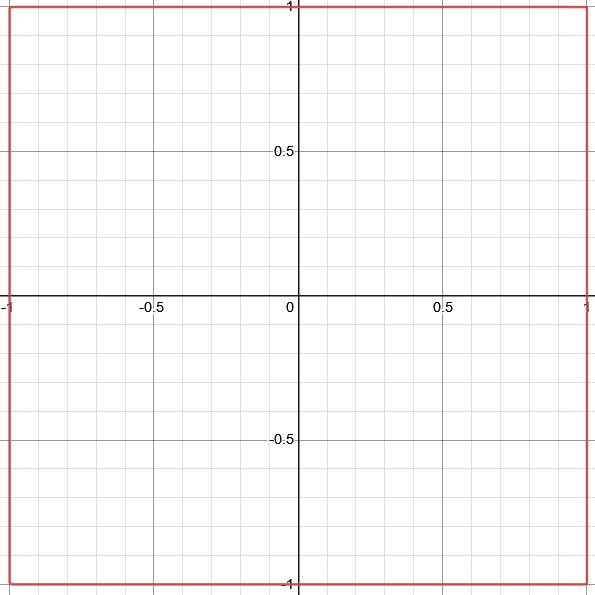
\includegraphics[scale=.75]{{images/linfinity_norm}.png}
\end{figure}
\newline

\end{enumerate}

\end{document}
